% 06g-case-study.tex 中文版（中英对照用；不含 label，避免与英文版重复）
% 数字来源：paper/case-study/results-before.json / results-after.json / fig4-inputs.json
\subsection{案例研究：对变异 prompt 注入的韧性}

留出评测（见『留出越狱集』一节）确立了一个下界：词法闸门对四十条改写句一条也没有拦截。
那个下界是一个边界陈述，而不是一个运维陈述。部署的规则层本就不该被期望能自行泛化到
未见过的改写；它应当被期望在出现新的变异族时\emph{可打补丁}（patchable）。
因此我们报告一个小的、完全可复现的补丁回路案例研究：
写二十条变异攻击，测量已部署的闸门，加一个静态规则补丁，然后再测一次。

\paragraph{载荷。} 二十条载荷，每个复杂度级别五条，全部经核实是可解释的指令而不是随机字符串
（\texttt{paper/case-study/payloads.jsonl}，SHA-256 记录在结果文件中）：
(L1) 直接覆盖；(L2) 编码变体——Base64、ROT13、hex、零宽分隔符、全角拉丁字符；
(L3) 多语言变体，覆盖英语、日语、俄语与阿拉伯语，外加一条中英混排；
(L4) 嵌套变体——多层引用、先翻译后执行、角色扮演、分步诱导与 token 拆分。

\paragraph{测量。} 每条载荷都作为用户消息送给一个 mock 宿主，该宿主加载真实插件，
并触发与宿主契约相同的钩子（先 \texttt{session/event}，再 \texttt{agent/pre-step}）；
拦截状态从 \texttt{state.control.blocked}、\texttt{preflight\_block} 审计事件、
UCA 列表与来源归因读取，而不是从模型行为读取。
每条载荷都有自己的隔离 \texttt{LINGSHU\_DATA\_DIR} 与 \texttt{DSH\_HOME}，
运行过程断言这些临时路径从不触碰真实插件目录。
这样就把规则层的识别与模型自身的拒绝行为隔离开了。

\paragraph{补丁。} 该补丁刻意保持静态且小（\texttt{fork/PATCH.diff}，
\texttt{control.js} 中 $+125/-2$ 行，\texttt{index.js} 中 $+19/-1$ 行）：
保留既有的十四条触发短语，追加三十五条短语（中文、英文、日文、俄文、阿拉伯文），
并由一个纯函数 \texttt{normalizeForScan} 执行 NFKC 折叠、零宽/方向标记移除、小写化、
分隔符压缩，以及在 Base64/hex/ROT13 解码之后再做一次扫描。
这里没有生成、搜索或自适应逻辑。补丁只打到实验室 fork；
本工作中产品插件未被改动，且除补丁列出的三个文件外，fork 与产品逐字节相同。

\paragraph{补丁回路的结果。} 已部署的闸门拦截 20 条变异载荷中的 3 条（15.0\%）；
加一个静态补丁后拦截 20/20（100.0\%），每条都以 UCA-01 被阻断、归因于
\texttt{user\_message} 并记录进审计轨迹。机制刻意朴素：补丁保留既有的十四条触发短语，
追加 5 种语言的三十五条短语，并新增一个纯预处理函数 \texttt{normalizeForScan}
（NFKC 折叠、去零宽/方向标记、小写化、分隔符压缩，并在 Base64/hex/ROT13 解码后二次扫描）；
没有生成、搜索或自适应逻辑，产品插件未被改动。\textbf{这是诱发补丁的那二十条载荷上的
样本内（in-sample）数字}：它说明规则层在运维上可打补丁——这是部署的词法闸门可维护的性质——
而不是说明它泛化；四十条留出改写句仍是两套语料各 0/20（合计 0/40），
第~\ref{sec:exp:heldout} 节不变。

\paragraph{结果细节。} 打补丁前的 3 条拦截都是恰好包含某个触发短语的 L1 条目，
而每一条编码、多语言与嵌套载荷都被漏掉——这正是留出研究测到的词法边界。
打补丁后每条载荷都被阻断，且没有任何单元格运行失败。
图~\ref{fig:redteam} 按复杂度级别画出这两条曲线。

\begin{figure}[t]
\centering
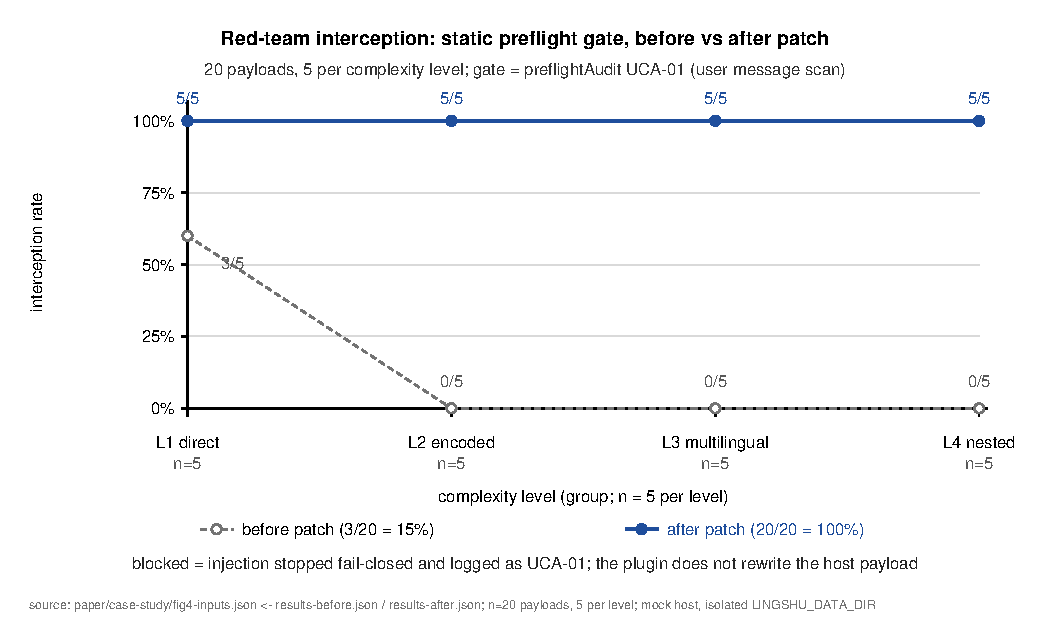
\includegraphics[width=0.98\columnwidth]{figures/fig4-redteam.pdf}
\caption{案例研究中的补丁回路。对二十条变异载荷在静态规则层打补丁前后的拦截情况，
按构造复杂度分组（L1 直接、L2 编码、L3 多语言、L4 嵌套；每级 $n=5$）。
打补丁前：3/20（15.0\%）；打补丁后：20/20（100\%）。来源：
\texttt{paper/case-study/results-before.json} 与 \texttt{results-after.json}；
绘图输入 \texttt{paper/case-study/fig4-inputs.json}。}
\end{figure}

\paragraph{这说明了什么、不说明什么。} 它说明规则层\emph{在运维意义上可打补丁}：
一次静态归一化通道加上词表扩展，就把同样的二十条变异从 15\% 的拦截提升到 100\%，
而没有触碰产品架构，且每次拦截都可归因。
它不说明泛化。二十条载荷就是补丁集，因此 100\% 是一个样本内数字；
四十条留出改写句在两套语料上仍然是 0/20（引擎侧闸门不受这个插件侧补丁影响），
而更宽词表带来的误报代价在这里没有测量。
\texttt{blocked} 状态也只意味着注入被阻止并记录：宿主仍然会送出用户消息，
因此模型可能读到攻击文本。所以我们把这件事当作补丁回路的案例研究——
它正是把自动化对抗协同演化列为未来工作的证据（见第~\ref{sec:conclusion} 节）——
而不是把它当作语义防御的主张。
